\chapter{Implicit One-Step Methods and Long-Term Stability}

\begin{intro}
  In the first chapter, we studied methods for the solution of IVP and
  the analysis of their convergence with shrinking step size $h$.  We
  could gain a priori error estimates from consistency and stability
  for sufficient small $h$.

  All of these error estimates are based on Grönwall's
  inequality. Therefore, they contain a term of the form $e^{Lt}$
  which increases fast with increasing length of the time interval
  $[t_0,T]$. Thus, the analysis is unsuitable for the study of
  long-term integration, since the exponential term will eventually
  outweigh any term of the form $h^p$.
  
  On the other hand, for instance our solar system has been moving on
  stable orbits for several billion years and we do not observe an
  exponential increase of velocities. Thus, there are in fact
  applications for which the simulation of long time periods is
  worthwhile and where exponential growth of the discrete solution
  would be extremely disturbing.
	
  This chapter first studies conditions on differential equations with
  bounded long term solutions, and then discusses numerical methods
  mimicking this behavior.
\end{intro}

%%%%%%%%%%%%%%%%%%%%%%%%%%%%%%%%%%%%%%%%%%%%%%%%%%%%%%%%%%%%%%%%%%%%%%
%%%%%%%%%%%%%%%%%%%%%%%%%%%%%%%%%%%%%%%%%%%%%%%%%%%%%%%%%%%%%%%%%%%%%%
\section{Monotonic initial value problem}
%%%%%%%%%%%%%%%%%%%%%%%%%%%%%%%%%%%%%%%%%%%%%%%%%%%%%%%%%%%%%%%%%%%%%%
%%%%%%%%%%%%%%%%%%%%%%%%%%%%%%%%%%%%%%%%%%%%%%%%%%%%%%%%%%%%%%%%%%%%%%

\begin{example}
  \label{ex:linear-model}
  We consider for $\lambda \in \C$ the linear initial value problem
  \begin{equation}
    \begin{split}
      \label{eq:impl:testproblem}
      u' & = \lambda u\\
      u(0) & = 1.
    \end{split}
  \end{equation}
  Splitting $\lambda=\Re(\lambda)+i\Im(\lambda)$ into its real and
  imaginary part, the (complex valued) solution to this problem is
  \begin{gather*}
     u(t) = e^{\lambda t}
     = e^{\Re(\lambda)t}\bigl(
     \cos(\Im(\lambda)t)+i\sin(\Im(\lambda)t)
     \bigr).
  \end{gather*}
  The behavior of $u(t)$ for $t\to\infty$ is determined by the real
  part of $\lambda$:
  \begin{gather}
    \label{eq:impl:cases}
    \begin{aligned}
      \Re(\lambda) < 0 & :\qquad& u(t) &\to 0 \\
      \Re(\lambda) = 0 & :\qquad& |u(t)| &= 1 \\
      \Re(\lambda) > 0 & :\qquad& u(t) &\to \infty
    \end{aligned}
  \end{gather}
  Moreover, the solution is bounded for $\lambda$ with non-positive
  real part for all points in time $t$.
\end{example}

\begin{remark}
  Since we deal in the following again and again with eigenvalues of
  real-valued matrices, we will always consider complex valued IVP
  hereafter, due to the well known fact, that these eigenvalues can be
  complex.
\end{remark}

\begin{remark}  
  Due to Grönwall's inequality and the stability
  \slideref{Theorem}{IVP-stability}, the solution to the IVP above
  admits the estimate $|u(t)| \le e^{|\lambda|t} |u(0)|$.  This is
  seen easily by applying the comparison function $v(t) \equiv 0$.  As
  soon as $\lambda \neq 0$ has a non-positive real part, this estimate
  is still correct but very pessimistic and therefore useless for
  large $t$.  Since problems with bounded long-term behavior are quite
  important in applications, we will have to introduce an improved
  notation of stability.
\end{remark}

\begin{Definition}{lipschitz-one-sided}
  \defindex{Lipschitz condition!one-sided}
  The function $f(t,y)$ satisfies on its domain $D \subset
  \R \times \C^d$ a \define{one-sided Lipschitz condition} if 
  the inequality
  \begin{gather}
    \label{eq:impl:Lipschitz}
    \Re \scal({f(t,y) - f(t,x)},y-x) \le \nu \abs{y-x}^2
  \end{gather}
  holds with a constant $\nu$ for all $(t,x),(t,y)\in D$. 
  Moreover such a function is called
  \textbf{monotonic} \defindex{monotonic function} if $\nu=0$, thus 
  \begin{gather}
    \label{eq:impl:monoton}
    \Re \scal({f(t,y) - f(t,x)},y-x) \le 0.
  \end{gather}
  An ODE $u'=f(u)$ is called monotonic if its right hand side $F$ is
  monotonic.
\end{Definition}

%%% Local Variables:
%%% mode: latex
%%% TeX-master: "../notes"
%%% End:


\begin{remark}
  The term monotonic from the previous definition is consistent with
  the term \emph{monotonically decreasing}, which we know from real-valued
  functions. We can see this by observing for $y>x$
  \begin{gather*}
    \bigl(f(t,y)-f(t,x)\bigr)(y-x) \le 0
    \quad \Leftrightarrow \quad f(t,y)-f(t,x) < 0.
  \end{gather*}
\end{remark}

\begin{Theorem}{stability-monotonic}
  Let $u(t)$ and $v(t)$ be two solutions of the equation
  \begin{gather*}
    u'=f(t,u),  \qquad v'=f(t,v),
  \end{gather*}
  with initial values $u(t_0) = u_0$ and $v(t_0) = v_0$,
  respectively. Let the function $f$ be continuous and let the
  one-sided Lipschitz condition~\eqref{eq:impl:Lipschitz} hold. Then
  we have for $t>t_0$:
  \begin{gather}
    \label{eq:implicit:3}
    \abs{v(t)-u(t)} \le e^{\nu(t-t_0)} \abs{v(t_0) - u(t_0)}.    
  \end{gather}
\end{Theorem}

%%% Local Variables:
%%% mode: latex
%%% TeX-master: "../notes"
%%% End:


\begin{proof}
  We consider the auxiliary function $m(t) = \abs{v(t)-u(t)}^2$ and
  its derivative
  \begin{align*}
    m'(t) &= 2\Re\scal({v'(t)-u'(t)},{v(t)-u(t)}) \\
    &= 2 \Re\scal({f\bigl(t,v(t)\bigr)-f\bigl(t,u(t)\bigr)},{v(t)-u(t)})
    \\
    &\le 2 \nu \abs{v(t)-u(t)}^2 \\
    &= 2 \nu m(t).
  \end{align*}
  According to Grönwall's inequality in \slideref{Lemma}{gronwall}
  we obtain for $t > t_0$:
  \begin{gather*}
    m(t) \le m(t_0) e^{2\nu(t-t_0)}.
  \end{gather*}
  Taking the square root yields the stability
  estimate~\eqref{eq:implicit:3}.
\end{proof}

\begin{remark}
  Analog to example~\ref{ex:linear-model} we obtain from the
  stability estimate, that for the difference of two solutions
  $u(t)$ and $v(t)$ of the differential equation $u'=f(t,u)$ we obtain 
	in the limit $t\to\infty$:
  \begin{gather}
    \label{eq:implicit:4}
    \begin{aligned}
      \nu < 0: & \qquad & \abs{v(t)-u(t)} &\to 0 \\
      \nu = 0: & \qquad & \abs{v(t)-u(t)} &\le \abs{v(t_0)-u(t_0)}
    \end{aligned}
  \end{gather}
\end{remark}

\begin{Lemma}{linear-monotonic}
  The linear differential equation $u'=Au$ with $u(t)\in \C^d$ and a
  diagonalizable matrix function $A(t) \in \C^{d\times d}$ admits the
  one-sided Lipschitz condition~\eqref{eq:impl:Lipschitz} with the
  constant
  \begin{gather*}
    \nu = \max_{\substack{i=1,\dots,d\\t\in \R}} \Re(\lambda_i).
  \end{gather*}
  Accordingly, this ODE is monotonic if and only if for all
  eigenvalues $\lambda_i$ of $A(t)$ there holds
  \begin{gather}
    \label{eq:implicit:10}
    \Re (\lambda_i) \le 0.
  \end{gather}
  This is the vector-valued form of example~\ref{ex:linear-model}. 
\end{Lemma}

\begin{proof}
  For the right hand side of the equation we have
  \begin{gather*}
    \Re \scal(A(t)y-A(t)x,y-x)
    \le \Re \frac{\scal(A(t)y-A(t)x,y-x)}{\abs{y-x}}\abs{y-x}
    \le \max_{i=1,\dots,d}\Re (\lambda_i) \abs{y-x}.
  \end{gather*}
  Hence, we obtain already $\nu \le \max_{i=1,\dots,d}
  \Re(\lambda_i)$. If we now insert for $x-y$ an eigenvector of 
	eigenvalue	$\lambda$ for which the maximum is accepted,
	then we obtain the equality and therefore $\nu = \max_{i=1,\dots,d}
  \Re(\lambda_i)$.
\end{proof}

%%%%%%%%%%%%%%%%%%%%%%%%%%%%%%%%%%%%%%%%%%%%%%%%%%%%%%%%%%%%%%%%%%%%%%
\subsection{Stiff initial value problems}
%%%%%%%%%%%%%%%%%%%%%%%%%%%%%%%%%%%%%%%%%%%%%%%%%%%%%%%%%%%%%%%%%%%%%%

\begin{example}
  \label{ex:impl:2}
  We consider the IVP
  \begin{gather}
    \label{eq:implicit:5}
    u' =
    \begin{pmatrix}
      -1 & 0 \\ 0 & -100
    \end{pmatrix}u,
    \qquad u(0) =
    \begin{pmatrix}
      1 \\ 1
    \end{pmatrix}.
  \end{gather}
  This has the solution
  \begin{gather*}
    u(t) =
    \begin{pmatrix}
      e^{-t} \\ e^{-100t}
    \end{pmatrix}.
  \end{gather*}
  We see, that the solution has a component which decreases slowly in
  time with $e^{-t}$ and a second one, which decreases fast with
  $e^{-100t}$. If we apply the Euler method with step size $h$ to this
  equation, then we obtain the method step
  \begin{gather*}
    y^{(n)} = y^{(n-1)} + h
    \begin{pmatrix}
      -1 & 0 \\ 0 & -100
    \end{pmatrix} y^{(n-1)}
    = \begin{pmatrix}
      1-h & 0 \\ 0 & 1-100h
    \end{pmatrix}y^{(n-1)}
  \end{gather*}
  with the solution
  \begin{gather*}
    y^{(n)} =
    \begin{pmatrix}
      (1-h)^n \\ (1-100h)^n
    \end{pmatrix}
  \end{gather*}
  If we are interested in the second solution component, the one which
  decreases fast, we choose $h$ to be small, say $h<1/100$. Thus, for
  $n\to\infty$ we have $y_n\to 0$, slowly in the first component, fast
  in the second one, just like the solution $u(t)$ of the continuous
  solution.  (Recall that for fixed chosen step size $h$ the limits
  $t\to\infty$ and $n\to\infty$ are equal.)
  
  If we are just interested in the first, the slow component, at a
  time where it has changed significantly.  then a considerably larger
  step size is appropriate, say $h=1/10$. For this step size the
  first solution component is still converging to zero with $y^{(n)}_1
  = 0.9^n$.  For the second one we have however $|y^{(n)}_2| =
  |(-9)^n| \to \infty$. Therefore the approximate solution for this
  step size diverges for $n\to\infty$, very much in contrast to the
  behavior of the exact solution $u(t)\to 0$ for $t\to\infty$.
\end{example}

\begin{remark}
  Of course, it would have been possible to ignore the second
  component in the previous example. But this is not a simple task in
  general, due to the fact that most solution components are
  coupled through the equation.  In such cases the step size of the
  Euler method must be chosen to accommodate the ``fast
  components''. This can lead to significant computational overhead.
  Therefore, we define in the following characteristic
  properties of such problems and develop to that specially adapted
  solution methods.
\end{remark}

\begin{Definition}{stiff}{Stiff IVP}
  \defindex{stiff initial value problem}
  \defindex{initial value problem!stiff}
  An initial value problem is called \define{stiff}, if it has
	the following characteristic properties:
  \begin{enumerate}
  \item The right hand side of the ODE is \putindex{monotonic}, or at
    least admits a one-sided Lipschitz condition with a small
    parameter $\nu$.
  \item The \putindex{time scales} on which the different solution
    components are evolving differ a lot, or in mathematical terms,
    the Lipschitz constant $L$ of the right hand side is greater than
    $\nu$ by orders of magnitude.
  \item The time scales which are of interest for the application 
    are much longer than the fastest time scales of the equation. Again
    in the language of our parameters: there is a constant $c$ of
    moderate size, such that
    \begin{gather}
      \label{eq:implicit:7}
      e^{LT} \le c e^{\nu T}.
    \end{gather}
  \end{enumerate}
\end{Definition}

%%% Local Variables:
%%% mode: latex
%%% TeX-master: "../notes"
%%% End:


\begin{remark}
  Even though we used the term definition, the notion of ``stiffness
  of an IVP'' has something vague or even inaccurate about it. In fact
  that is due to the very nature of the problems and cannot be fixed.
  Instead we are forced to sharpen our understanding by means of a few
  examples.
\end{remark}

\begin{remark}
  The third condition in the definition of stiffness is rather rare to
  find in the literature, but it is in general implicitly assumed by
  the discussion for time step methods for stiff IVP.  It is important
  though to realize, that the methods of the previous chapter do not
  cause problems computing a good resolution for the fastest time
  scales. In this case, $e^{Lt}$ will be not too much greater than
  $e^{\nu t}$.
\end{remark}

\begin{example}
  \label{ex:impl:2a}
  First of all we will have a look at equation~\eqref{eq:implicit:5}
  in example~\ref{ex:impl:2}. The first condition of the stiffness
  definition is fulfilled. The decrease to $1/e$ happens at $t=1$ and
  at $t=1/100$ for the first and second component, respectively.
  Thus, the second condition holds as well.
  
  According to the discussion of example~\ref{ex:impl:2}, the third
  condition depends on the purpose of the computation.  If we want
  to compute the solution at time $t=1/100$, we would not denote the
  problem as stiff. As one is interested on the solution at time
  $t=1$, on which the second component with $e^{-100}$ is already
  below typical machine accuracy, the problem is stiff indeed. Here
  we have seen that Euler's method requires disproportionately small
  time steps.
\end{example}

\begin{remark}
  \label{remark:impl:1}
  The definition of stiffness and the discussion of the examples
  reveal that numerical methods are needed, which are not just
  convergent for time steps $h\to 0$ but also for fixed step size $h$,
  even in the presence of time scales clearly below $h$. In this case,
  methods still have to produce solutions with correct limit behavior
  for $t\to\infty$.
\end{remark}

\begin{example}
  The \define{implicit Euler method} is defined by the one-step
  formula
  \begin{gather}
    \label{eq:implicit:17}
    y_1 = y_0 + hf(t_1, y_1)
    \quad \Leftrightarrow \quad
    y_1 - h f(t_1, y_1) = y_0.
  \end{gather}
  Applied to our example~\eqref{eq:implicit:5}, we observe
  \begin{gather*}
    y^{(n)} =
    \begin{pmatrix}
      1 + h & 0 \\ 0 & 1+100h
    \end{pmatrix}^{-1}
    y^{(n-1)}.
  \end{gather*}
  This yields the solution
  \begin{gather*}
    y^{(n)} =
    \begin{pmatrix}
      \frac1{(1+h)^n} \\
      \frac1{(1+100h)^n}
    \end{pmatrix}
  \end{gather*}
  which converges to zero for $n\to \infty$, independent of $h$. Thus,
  although the implicit Euler method requires in general the solution
  of a nonlinear system in each step, it allows for much larger time
  steps than the explicit Euler method,when applied to a stiff problem.
  
  For a visualization of the implicit and explicit Euler method see the
  appendix.
\end{example}
%%%%%%%%%%%%%%%%%%%%%%%%%%%%%%%%%%%%%%%%%%%%%%%%%%%%%%%%%%%%%%%%%%%%%%
%%%%%%%%%%%%%%%%%%%%%%%%%%%%%%%%%%%%%%%%%%%%%%%%%%%%%%%%%%%%%%%%%%%%%%
\section{A- and B-stability}
%%%%%%%%%%%%%%%%%%%%%%%%%%%%%%%%%%%%%%%%%%%%%%%%%%%%%%%%%%%%%%%%%%%%%%
%%%%%%%%%%%%%%%%%%%%%%%%%%%%%%%%%%%%%%%%%%%%%%%%%%%%%%%%%%%%%%%%%%%%%%

\begin{intro}
  In this section, we will investigate desirable properties of
  one-step methods for stiff IVP~\eqref{eq:implicit:6}. We will first
  study linear problems of the form
\begin{gather}
  \label{eq:implicit:6}
  u'=Au \qquad u(t_0) = u_0.
\end{gather}
and the related notion of A-stability in
  detail From the conditions for stiffness we derive the following
  problem characteristics:
  \begin{enumerate}
  \item All eigenvalues of the matrix $A$ lie in the left half-plane
    of the complex plane. With~\eqref{eq:impl:cases} all solutions are
    bounded for $t\to\infty$.
  \item There are eigenvalues close to zero and eigenvalues with a
    large negative real part.
  \item We are interested in time spans which make it necessary, that
    the product $h\lambda$ of a time step and an arbitrary eigenvalue,
    is allowed to be large.
  \end{enumerate}
  For this case we now want to derive criteria for the boundedness of
  the discrete solution for $t\to\infty$. The important part is not to
  derive an estimate holding for $h\to 0$, but one that holds for any
  value of $h\lambda$ in the left half-plane of the complex numbers.
\end{intro}

\begin{Definition}{stability-function}
  The \define{stability function} $R(z) = R(h \lambda)$ is the
  function generated by applying the one-step method
  \begin{gather*}
    y_1 = y_0 + h \verfahren_h(t_0, y_0)
  \end{gather*}
  to the linear test problem $u'(t)=\lambda u(t)$. Therefore,
  \begin{equation}
    y_1 = R(h \lambda) u_0,
  \end{equation}
  and
  \begin{equation}
    y^{(n)} = R(h \lambda)^n u_0.
  \end{equation}
  The \define{stability region} of a one-step method is the set
  \begin{gather}
    S = \bigl\{ z \in \C \big| \abs{R(z)} \le 1 \bigr\}.
  \end{gather}
\end{Definition}

\begin{example}
  The stability function of the explicit Euler method is derived as follows:
  \begin{equation}\begin{split}
      \label{eq:impl:stabil:expleuler}
      y_1 &= y_0 + h \lambda y_0 = (1 + h \lambda) y_0 \\
      \Rightarrow R(h \lambda) &= 1 + h \lambda \\
      R(z) &= 1 + z \\
    \end{split}\end{equation}
  The stability region for the explicit Euler is a circle with radius
  1 around the point (-1,0) in the complex plane (see Figure~\ref{fig:implicit:stability-euler})
\end{example}


\begin{example}
  The stability function of the implicit Euler method is derived as follows:
  \begin{equation}\begin{split}
  \label{eq:impl:stabil:impleuler}
    y_1 &= y_0 + h f(t_1, y_1) \\
    y_1 &= y_0 + h \lambda y_1 \\
    (1 - h \lambda) y_1 &= y_0 \\
    \Rightarrow R(h \lambda) &= \frac{1}{1- h \lambda} \\
    R(z) &= \frac{1}{1-z} \\
  \end{split}\end{equation}
The stability region for the implicit Euler is the complement of a
circle with radius 1 around the point (1,0) in the complex plane (see
Figure~\ref{fig:implicit:stability-euler}). %% anschauliches Bild?
\end{example}
\begin{figure}[tp]
  \centering
  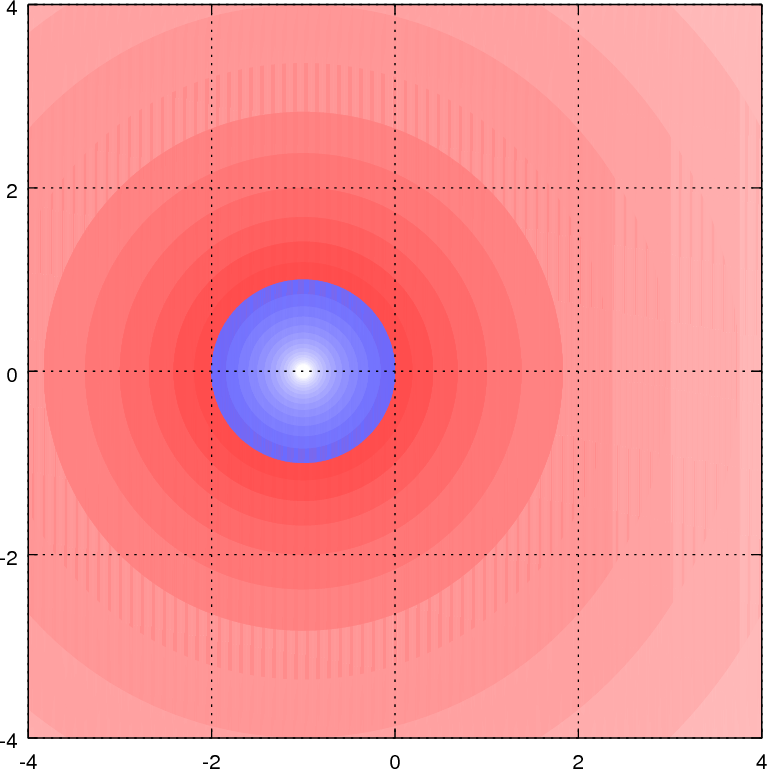
\includegraphics[width=.47\textwidth]{fig/stability-euler}
  \hfill
  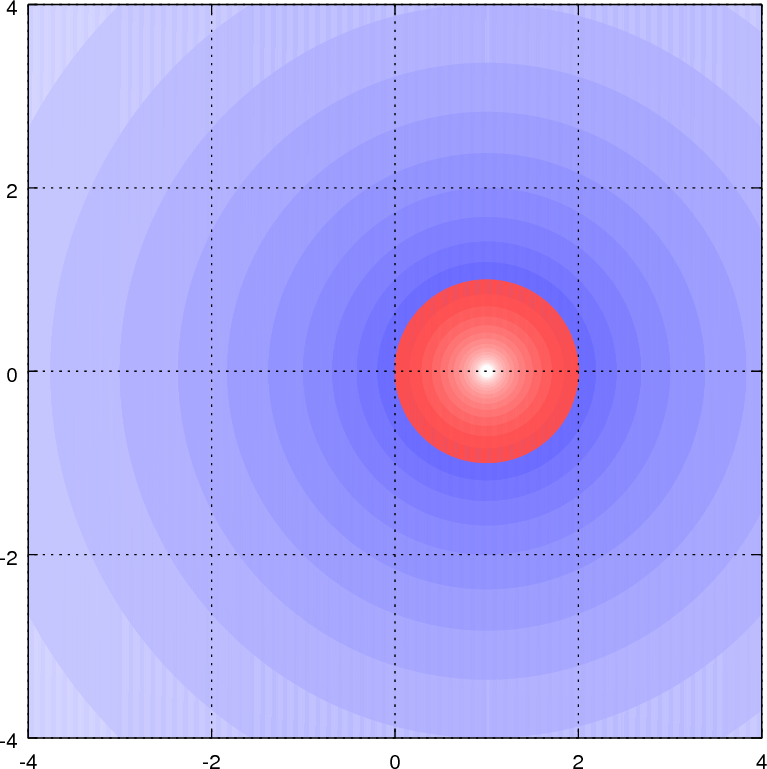
\includegraphics[width=.47\textwidth]{fig/stability-euler2}
  \caption{Stability regions of the explicit and implicit Euler
    methods (blue stable, red unstable)}
  \label{fig:implicit:stability-euler}
\end{figure}

\begin{Definition*}{a-stability}{A-stability}
  A method is called \define{A-stable}, if its stability region contains
  the left half-plane of $\C$, hence
  \begin{gather}
    \{ z \in \C | \Re(z) \le 0 \} \subset S
  \end{gather}
\end{Definition*}

\begin{Theorem}{a-stability}
  Let $\left\{y^{(k)}\right\}$ be the sequence generated by an
  A-stable one-step method of step size $h$ for the linear, autonomous IVP
  \begin{gather*}
    u'=Au, \qquad u(t_0) = u_0
  \end{gather*}
  with a diagonalizable matrix $A$ an initial value $y^{(0)} =
  u_0$. If additionally all eigenvalues of $A$ have a non-positive
  real part, then the sequence members $y^{(k)}$ are uniformly bounded
  for all $h$.
\end{Theorem}

 \begin{remark}
  The notion of A-stability was deliberately chosen neutrally by Dahlquist.
  In particaluar, note that A-stability does not stand for asymptotic stability.
 \end{remark}

\begin{proof}
  Let $\{v_\ell\}_{\ell=1,\dots,d}$ be a basis of $\C^d$ consisting of
  eigenvectors of $A$. Such a basis exists since $A$ is
  diagonalizable. Let $y_0 = \sum_{\ell=1}^d \alpha^\ell v_\ell$ be
  the representation of $y_0$ in this basis. Furthermore, we introduce
  the representations $g_i = \sum_{\ell=1}^d \gamma_i^\ell
  v_\ell$. Then, we see that equations of the form
  \begin{gather*}
    g_i = y_0 + h \sum_{j=1}^s a_{ij} A g_i
  \end{gather*}
  decouple into
  \begin{gather*}
    \gamma_{i}^\ell = \alpha^\ell + h \sum_{j=1}^s a_{ij} \lambda_\ell \gamma_j^\ell.
  \end{gather*}
  Similarly, if $y_1 = \sum_{\ell=1}^d \eta^\ell v_\ell$ we have the separation
  \begin{gather*}
    y_1 = y_0 + h\sum_{i=1}^s b_i g_i
    \quad\longrightarrow\quad
    \eta^\ell = \alpha^\ell  + h\sum_{i=1}^s b_i \gamma_i^\ell.
  \end{gather*}
  Thus, instead of a vector valued problem, the method solves $d$
  decoupled scalar problems, inside and across time steps. But for each of the scalar problems, the definition of A-stability implies boundedness of the solution, if $\Re(\lambda_\ell) \le 0$.
\end{proof}

\begin{Theorem}{implicit:a-stability-erk}
  No explicit Runge-Kutta method is A-stable.
\end{Theorem}

\begin{proof}
  We show that for such methods $R(z)$ is a polynomial.  Then, the
  theorem follows immediately, it is known for polynomials, that the
  absolute value of its values goes to infinity, if the absolute value
  of the argument goes to infinity.
  
  From the equation~\eqref{eq:explicit:1b} follows $k_i = \lambda
  g_i$. If we insert that into the equation~\eqref{eq:explicit:1a},
  we obtain
  \begin{gather*}
    g_i = y_0 + h \sum_{j=1}^{i-1} \rka_{ij}k_j = y_0 + h\lambda
    \sum_{j=1}^{i-1} \rka_{ij} g_j.
  \end{gather*}
  With $g_1 = y_0$ and $z=h\lambda$ one has
  \begin{align*}
    g_2 &= y_0+ \rka_{21} z y_0 = (1+\rka_{21}z) y_0\\
    g_3 &= y_0 +  \rka_{32} z g_2 =  y_0 +  \rka_{32} z (1+\rka_{21} z) y_0 =
    (1+\rka_{32} z(1+\rka_{21} z)) y_0.
  \end{align*}
	Therefore one shows easily per induction that $k_j$ results as
	multiplication of a polynomial of order $j-1$ with $y_0$. 
  With formula~\eqref{eq:explicit:1c} we have that $R(z)$ is a
  polynomial of order $\rks-1$.
\end{proof}



\begin{remark}
  The notion of A-stability is only applicable to linear problems with
  diagonalizable matrices. Now we are considering its extension to
  nonlinear problems with monotonic right hand sides.
\end{remark}

\begin{Definition}{b-stability}
  A one-step method is called \define{B-stable}, if for monotonic
  initial value problems $u'=f(u)$ with arbitrary initial value $y_0$
  and $z_0$ there holds:
  \begin{equation}
    | y_1 - z_1 | \le | y_0 - z_0 |
  \end{equation}
  independent of the time step size $h$.
\end{Definition}


\begin{Theorem}{b-stability}
  Let be $\left\{y^{(k)}\right\}$ the sequence generated by a
  B-stable method for the IVP
  \begin{gather*}
    u'=f(u), \qquad u(t_0) = u_0
  \end{gather*}
  with initial values $y^{(0)} = u_0$. If the right hand side $f$ is
  monotonic, then the values $y^{(k)}$ of the sequence are uniformly
  bounded for for $k\to\infty$ independent of the time step size $h$.
\end{Theorem}

\begin{proof}
  The theorem follows immediately by iterating over the definition of
  B-stability.
\end{proof}

\begin{Corollary}{b-stable-a-stable}
  A B-stable method is A-stable.
\end{Corollary}

\begin{proof}
  Apply the method to the linear differential model equation, which is
  monotonic for $\Re(\lambda) \le 0$. Now, the definition of B-stability
  implies $\abs{R(z)} \le 1$, and thus, the method is A-stable.
\end{proof}

\subsection{L-stability}

An undesirable feature of complex differentiable functions in the
context of stability of Runge-Kutta methods is the fact, that the
limit $\lim_{z\to \infty} R(z)$ is well-defined on the \putindex{Riemann sphere},
independent of the
path chosen to approach this limit in the complex plane. Thus, for any
real number $x$, we have
\begin{gather}
  \lim_{x\to\infty} R(x) = \lim_{x\to\infty} R(ix).
\end{gather}

Thus, a method, which has exactly the left half-plane of $\C$ as its
stability domain, seemingly a desirable property, has the undesirable
property that components in eigenspaces corresponding to very large
negative eigenvalues, and thus decaying very fast in the continuous
problem, are decaying very slowly if such a method is applied.

This gave raise to the following notion of L-stability. We
nevertheless point out, that the L-stable methods are not always to be
considered better than A-stable ones, like it is not always necessary
to require A-stability. Judgment must be applied according to the
problem being solved.

\begin{Definition}{l-stability}
  An A-stable one-step method is called \define{L-stable}, if for its
  \putindex{stability function} there holds
  \begin{gather}
    \lim_{\Re (z) \to -\infty} \abs{R(z)} = 0.
  \end{gather}
  Some authors refer to L-stable methods as \define{strongly A-stable}.
\end{Definition}

%%%%%%%%%%%%%%%%%%%%%%%%%%%%%%%%%%%%%%%%%%%%%%%%%%%%%%%%%%%%%%%%%%%%%%
%%%%%%%%%%%%%%%%%%%%%%%%%%%%%%%%%%%%%%%%%%%%%%%%%%%%%%%%%%%%%%%%%%%%%%
\section{General Runge-Kutta methods}
%%%%%%%%%%%%%%%%%%%%%%%%%%%%%%%%%%%%%%%%%%%%%%%%%%%%%%%%%%%%%%%%%%%%%%
%%%%%%%%%%%%%%%%%%%%%%%%%%%%%%%%%%%%%%%%%%%%%%%%%%%%%%%%%%%%%%%%%%%%%%

\begin{intro}
  According to theorem~\ref{Theorem:implicit:a-stability-erk}, ERK
  cannot be A- or B-stable. Thus, they are not suitable for long term
  integration of stiff IVP. The goal of this chapter is the study of
  methods not suffering from this limitation. The cure will be
  implicit methods, where stages may not only depend on
  known values from the past, but also on the value to be computed.
  
  We point out at the beginning of this chapter, that the main
  drawback of these methods is the fact that they require the solution
  of a typically nonlinear system of equations and thus involve much
  higher computational effort. Therefore, careful judgment should
  always be applied to determine whether a problem is really stiff or
  an implicit method is needed for other reasons.
\end{intro}

\begin{Definition}{rk}
  A \define{Runge-Kutta method} is a one-step method of the form
  \begin{subequations}
    \label{eq:implicit:1}
    \begin{xalignat}{2}
      \label{eq:implicit:1a}
      \rkg_i &= y_0 + h \sum_{j=1}^{\rks} \rka_{ij} k_j
      & i &= 1,\dots,\rks
      \\
      \label{eq:implicit:1b}
      k_i &= f(t_0+h \rkc_i, \rkg_i)
      & i &= 1,\dots,\rks
      \\
      \label{eq:implicit:1c}
      y_1 &= y_0 + h \sum_{i=1}^{\rks} \rkb_i k_i
    \end{xalignat}
  \end{subequations}
  The method is called
  \begin{description}
  \item[\textbf{ERK}] if $j \ge i\Rightarrow\rka_{ij} = 0$ (``explicit'')
    \index{Runge-Kutta method!explicit (ERK)|textbf}
  \item[\textbf{DIRK}] if $j>i\Rightarrow\rka_{ij} = 0$ (``diagonal implicit'')
    \index{Runge-Kutta method!diagonal implicit (DIRK)|textbf}
    \index{Diagonal implicit (DIRK)}
    \index{DIRK|see{Runge-Kutta method}}
  \item[\textbf{SDIRK}] if DIRK and $\forall i,j: \rka_{ii} =
    \rka_{jj}$ (``singly diagonal implicit'')
    \index{Runge-Kutta method!singly diagonal implicit (SDIRK)|textbf}
    \index{SDIRK|see{Runge-Kutta method}}
  \item[\textbf{IRK}] ``implicit'' in all other cases.
    \index{Runge-Kutta method!implicit (IRK)|textbf}
    \index{IRK|see{Runge-Kutta method}}
  \end{description}
\end{Definition}

%%% Local Variables: 
%%% mode: latex
%%% TeX-master: "../notes"
%%% End: 



\begin{example}[Two-stage SDIRK]
  Both SDIRK methods in table~\ref{tab:SDIRK2} are of 
  order three
  \begin{table}[htp]
    \centering
  \begin{gather}
    \def\arraystretch{1.5}
    \begin{array}{c|cc}
      \frac12 - \frac{\sqrt{3}}{6} & \frac12 - \frac{\sqrt{3}}{6} & 0 \\
      \frac12 + \frac{\sqrt{3}}{6} & \frac{\sqrt{3}}{3} & \frac12 - \frac{\sqrt{3}}{6} \\
      \hline
      & \frac12 & \frac12
    \end{array}
    \qquad
    \begin{array}{c|cc}
      \frac12 + \frac{\sqrt{3}}{6} & \frac12 + \frac{\sqrt{3}}{6} & 0 \\
      \frac12 - \frac{\sqrt{3}}{6} & -\frac{\sqrt{3}}{3} & \frac12 + \frac{\sqrt{3}}{6} \\
      \hline
      & \frac12 & \frac12
    \end{array}
  \end{gather}
    \caption{Two-stage SDIRK method of order 3}
    \label{tab:SDIRK2}
  \end{table}
\end{example}

% HW2, p. 40
\begin{Lemma}{stability-rk}
  The \putindex{stability function} of an $s$-stage Runge-Kutta method with
  coefficients
  \begin{gather*}
    A=
    \begin{pmatrix}
      \rka_{11} & \cdots & \rka_{1s}
      \\ \vdots & & \vdots \\
      \rka_{s1} & \cdots & \rka_{ss}
    \end{pmatrix},
    b =
    \begin{pmatrix}
      b_1 \\ \vdots \\ b_s
    \end{pmatrix},
  \end{gather*}
  is given by the two expressions
  \begin{gather}
    \label{eq:stability-rk:1}
    R(z) = 1+ z b^T \bigl(\identity-zA\bigr)^{-1}
    \begin{pmatrix}
      1\\\vdots\\1
    \end{pmatrix}
    = \frac{\operatorname{det}\left(\identity-zA+z
        \begin{pmatrix}
          b_1 & \cdots & b_s\\
          \vdots & & \vdots \\
          b_1 & \cdots & b_s
        \end{pmatrix}\right)
}{\operatorname{det}\bigl(\identity-zA\bigr)}
  \end{gather}
\end{Lemma}

%%% Local Variables:
%%% mode: latex
%%% TeX-master: "../notes"
%%% End:


\begin{proof}
  Entering $f(u) = \lambda u$ into the definition of the stages $g_i$,
  we obtain the linear system
  \begin{gather*}
    g_i = y_0 + h \sum_{j=1}^s a_{ij}\lambda g_j, \quad i=1,\dots,s.
  \end{gather*}
  In matrix notation with $z=h\lambda$, we obtain
  $(\identity-z A) g = (y_0,\dots,y_0)^T$, where $g$ is the vector
  $(g_1,\dots,g_s)^T$. Equally, we obtain
  \begin{align*}
    R(z) y_0 = y_1 &= y_0 + h \sum_{i=1}^s b_i \lambda g_i = y_0 + z
    b^T g\\
    &= y_0 + z b^T(\identity-z A)^{-1}
    \begin{pmatrix}
      y_0\\\vdots\\y_0
    \end{pmatrix}
    \\
    &= \left(1+z b^T(\identity-z A)^{-1}
      \begin{pmatrix}
        1\\\vdots\\1
      \end{pmatrix}
    \right) y_0.
  \end{align*}
  In order to prove the second representation, we write the whole Runge-Kutta method
  as a single system of equations of dimension $s+1$:
  \begin{gather*}
    \begin{pmatrix}
      I-z A & 0 \\
      -z b^T & 1
    \end{pmatrix}
    \begin{pmatrix}
      g \\ y_1
    \end{pmatrix}
    = y_0
    \begin{pmatrix}
      1\\\vdots\\1
    \end{pmatrix}.
  \end{gather*}
  Applying Cramer's rule yields the result.
\end{proof}

\begin{Example}{stability-examples-rk}
  Stability functions of the modified Euler method, of the classical
  Runge-Kutta method of order 4 and of the Dormand-Prince method of
  order 5 are
  \begin{align*}
    R_2(z) &= 1 + z + \tfrac{z^2}2 \\
    R_4(z) &= 1 + z + \tfrac{z^2}2 + \tfrac{z^3}{6} + \tfrac{z^4}{24}\\
    R_5(z) &= 1 + z + \tfrac{z^2}2 + \tfrac{z^3}{6} + \tfrac{z^4}{24}
             + \tfrac{z^5}{120} + \tfrac{z^6}{600}
  \end{align*}
  respectively. Their stability regions are shown in
  Figure~\ref{fig:implicit:stability-explicit-rk}.
\end{Example}

%%% Local Variables:
%%% mode: latex
%%% TeX-master: "../notes"
%%% End:

\begin{figure}[tp]
  \centering
  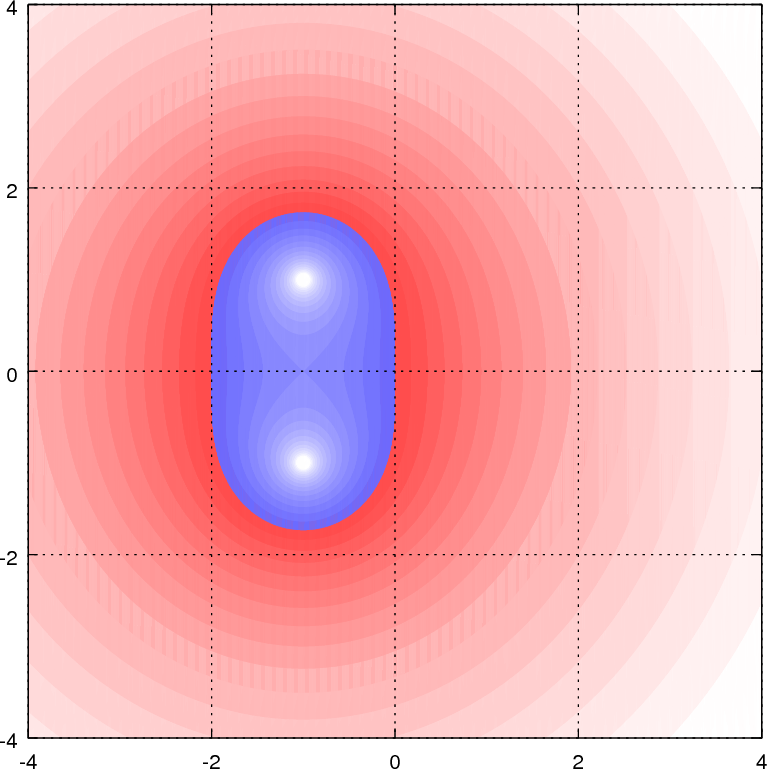
\includegraphics[width=.3\textwidth]{fig/stability-RK2}
  \hfill
  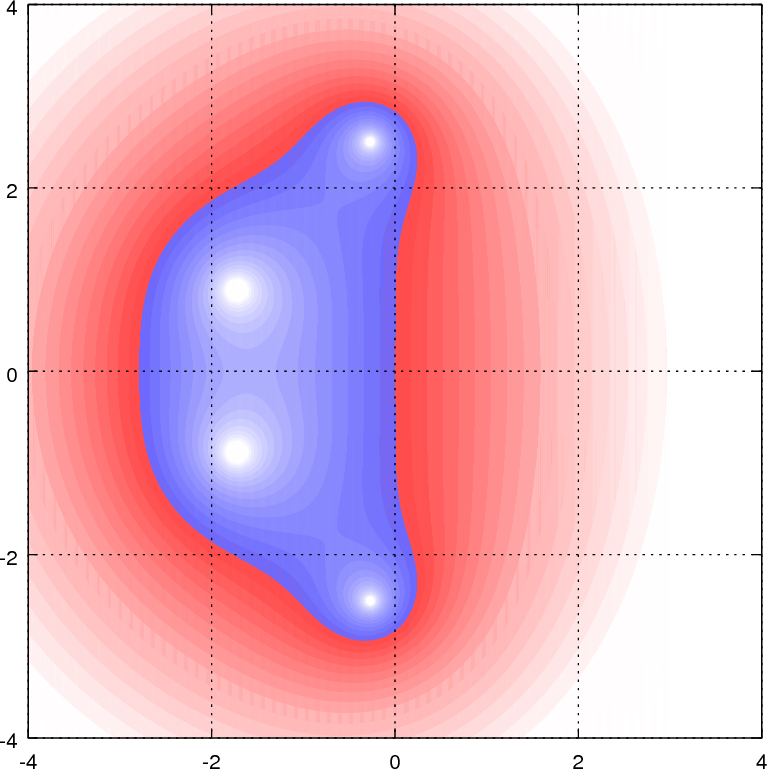
\includegraphics[width=.3\textwidth]{fig/stability-RK4}
  \hfill
  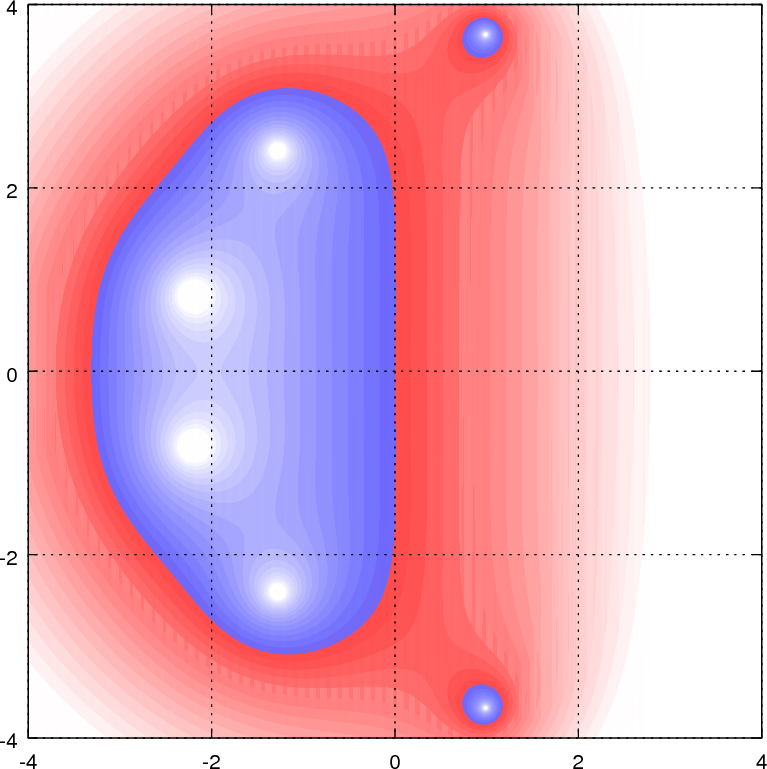
\includegraphics[width=.3\textwidth]{fig/stability-DOPRI5}
  \caption{Stability regions of the modified Euler method, the
    classical Runge-Kutta method of order 4 and the Dormand/Prince
    method of order 5 (blue stable, red unstable)}
  \label{fig:implicit:stability-explicit-rk}
\end{figure}

\begin{Definition}{theta-scheme}
  The $\theta$-scheme is the one-step method, defined for $\theta\in
  [0,1]$ by
  \begin{gather}
    \label{eq:theta:1}
    y_1 = y_0 + h \bigl((1-\theta) f(y_0) + \theta f(y_1)\bigr).
  \end{gather}
  It is an RKM with the Butcher Tableau
  \begin{gather}
    \label{eq:theta:2}
    \begin{array}{c|cc}
      0 & 0 & 0 \\
      1 & 1-\theta & \theta \\\hline
      & 1-\theta & \theta
    \end{array}.
  \end{gather}
  Three special cases are distinguished:
  \begin{center}
  \begin{tabular}{c|l}
    $\theta=0$ & explicit Euler method\\
    $\theta=1$ & implicit Euler method\\
    $\theta=1/2$ & Crank-Nicolson method
  \end{tabular}    
  \end{center}

  Furthermore, we define the variable $\theta$-scheme where $\theta$ is
  of the form
  \begin{gather*}
    \theta = \frac12 + \gamma h.
  \end{gather*}
\end{Definition}
%%% Local Variables:
%%% mode: latex
%%% TeX-master: "../notes"
%%% End:


\begin{Theorem}{theta-a-stability}
  The $\theta$-scheme is A-stable for $\theta\ge 1/2$. Furthermore, if
  there exists a constant $c$ such that $\theta-1/2 \le ch$, the
  method is consistent of second order.
\end{Theorem}

\begin{proof}
  Left as a homework question. Additionally, we show stability regions
  for different $\theta$ in figure ~\ref{fig:implicit:theta}.
  \begin{figure}[tp]
    \centering
    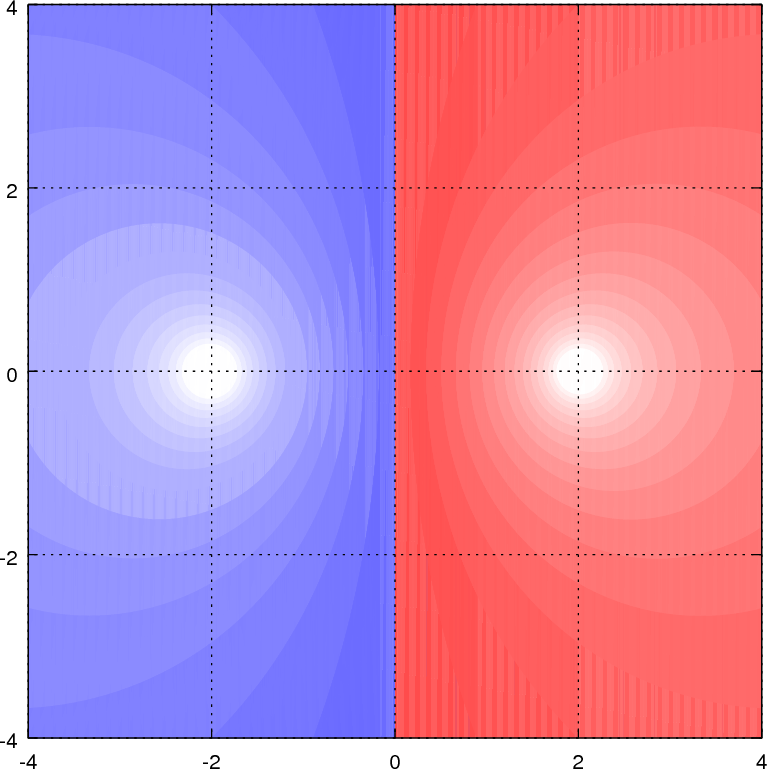
\includegraphics[width=.45\textwidth]{fig/stability-CR}
    \hfill
    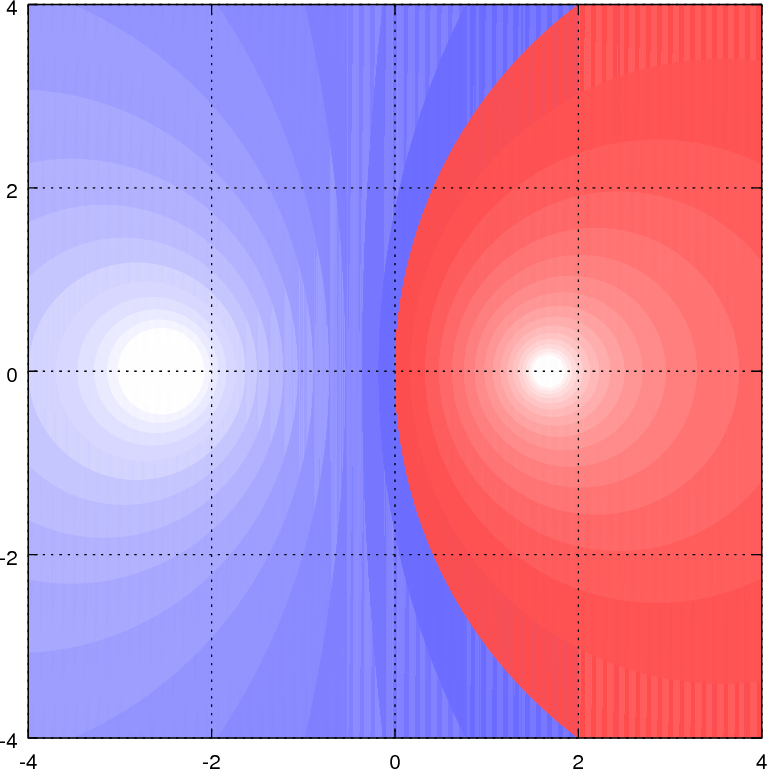
\includegraphics[width=.45\textwidth]{fig/stability-theta6}

    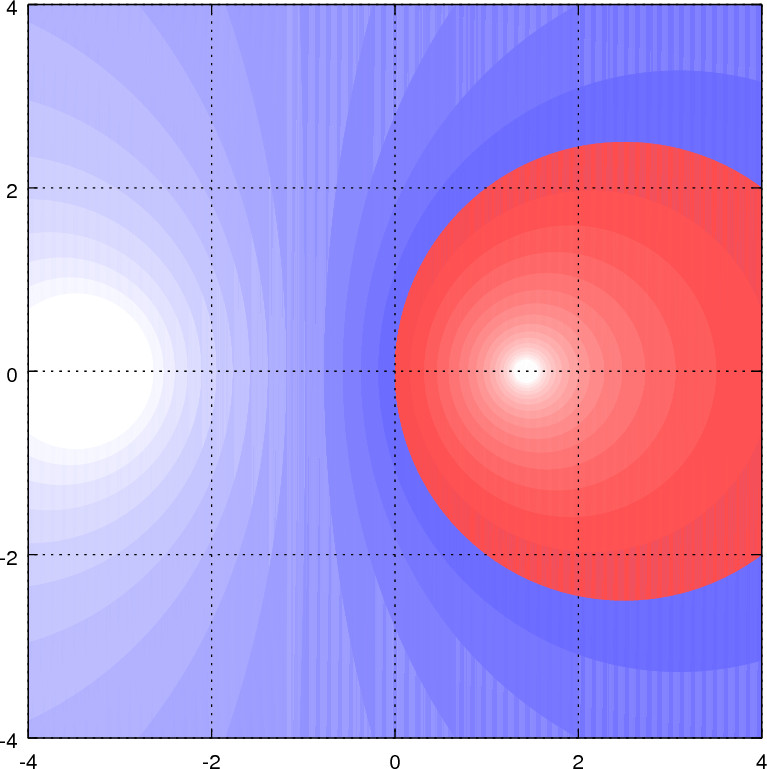
\includegraphics[width=.45\textwidth]{fig/stability-theta7}
    \hfill
    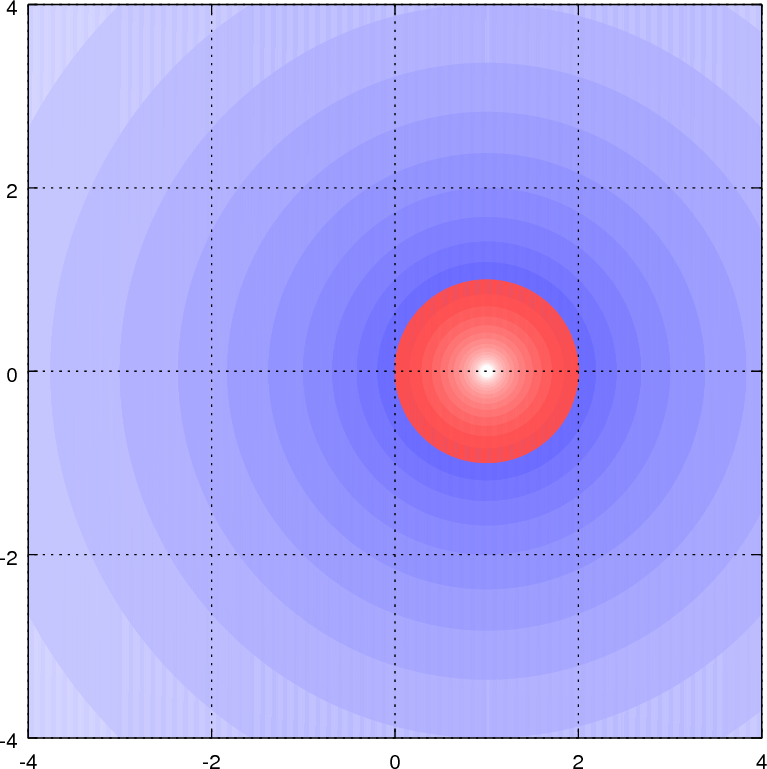
\includegraphics[width=.45\textwidth]{fig/stability-euler2}
    \caption{Stability regions of the $\theta$-scheme with
      $\theta=0.5$ (Crank-Nicolson), $\theta=0.6$, $\theta=0.7$, and
      $\theta=1$ (implicit Euler).}
    \label{fig:implicit:theta}
  \end{figure}
\end{proof}

\subsection{Existence and uniqueness of discrete solutions}

While it was clear that the steps of an explicit Runge-Kutta method
can always be executed, implicit methods require the solution of a
possibly nonlinear system of equations. The solvability of such a
system is not always clear. We will investigate several cases here:
First, Lemma~\ref{Lemma:existence-implicit-1} based on a Lipschitz
condition on the right hand side. Since this result suffers from a
severe step size constraint, we add
Lemma~\ref{Lemma:existence-implicit-2} for DIRK methods based on right
hand sides with a one-sided Lipschitz condition. Finally, we present
Theorem~\ref{Theorem:existence-implicit-3} for general Runge-Kutta
methods with one-sided Lipschitz condition.

\begin{Lemma}{existence-implicit-1}{Cauchy 1824}
  Let $f:\R\times\C^d\to\C^d$ be continuous and satisfy the Lipschitz
  condition with constant $L$. If
  \begin{gather}
    \label{eq:existence-implicit-1:1}
    hL < \frac1{\max\limits_{i=1,\dots,s} \sum\limits_{j=1}^s \abs{a_{ij}}},
  \end{gather}
  then, for any $y_0$ the Runge-Kutta method~\eqref{eq:implicit:1} has a unique
  solution $y_1$.
\end{Lemma}

%%% Local Variables:
%%% mode: latex
%%% TeX-master: "../notes"
%%% End:


\begin{proof}
  We prove existence and uniqueness by a fixed-point argument. To this
  end, define the vectors
  $k^{(m)}=(k_1^{(m)},\dots,k_s^{(m)})^T\in \R^{s d}$ for $m=1,\dots$
  and the iteration $k^{(m)} = F(k^{(m-1)}$ by
  \begin{gather*}
    k_i^{(m)} = F_i(k^{(m-1)}) = f\left(
      t_0+c_i h, y_0+ h \sum_{j=1}^s a_{ij} k_j^{(m-1)}\right),
    \quad i=1,\dots,s.
  \end{gather*}
  Clearly the vector $k=(k_1,\dots,k_s)^T\in \R^{s d}$ of the
  Runge-Kutta method is a fixed-point of this iteration. Using on
  $\R^{s d}$ the norm $\norm{k} = \max_{i=1,\dots,s} \abs{k_i}$, where
  $\abs{.}$ is the regular Euclidean norm on $\R^d$, we obtain the
  estimate
  \begin{gather*}
    \norm{F(k_1)-F(k_2)}
    \le  \left(h L \max_{i=1,\dots,s} \sum_{j=1}^s \abs{a_{ij}}\right)
    \norm{k_1-k_2}.
  \end{gather*}
  Under assumption~\eqref{eq:existence-implicit-1:1}, the term in
  parentheses is strictly less than unity and thus, the mapping $F$ is
  a contraction. The \putindex{Banach fixed-point theorem} yields the
  unique existence.
\end{proof}

\begin{Lemma}{existence-implicit-2}
  Let $f:\R\times\C^d\to\C^d$ be continuous and satisfy the one-sided Lipschitz
  condition with constant $\nu$. If for $i=1,\dots,s$
  \begin{gather}
    \label{eq:existence-implicit-2:1}
    h\nu < \frac1{a_{ii}}
  \end{gather}
  then, for any $y_0$ the DIRK method~\eqref{eq:implicit:1} has a unique
  solution $y_1$.
\end{Lemma}

%%% Local Variables:
%%% mode: latex
%%% TeX-master: "../notes"
%%% End:


\begin{proof}
  The proof simplifies compared to the general case of an IRK, since
  each stage depends explicitly on the previous stages and implicitly
  only on itself.  Thus, we can write
  \begin{gather}
    \label{eq:implicit:18}
    g_i = y_0 + v_i + h a_{ii} f(g_i),
    \quad\text{with}\quad
    v_i = h \sum_{j=1}^{i-1} a_{ij} f(g_j).
  \end{gather}
  For linear IVP with diagonalizable matrix $A$, we have
  \begin{gather*}
    \left(I-ha_{ii} A\right) g_i = y_0 + v_i,
  \end{gather*}
  and assumption~\eqref{eq:existence-implicit-2:1} implies that all
  eigenvalues of $\left(I-ha_{ii} A\right)$ are positive, thus, the
  inverse exists and we obtain a unique solution.

  In the nonlinear case, we use a homotopy argument. To this end, we
  introduce the parameter $\tau\in [0,1]$ and set up the family of
  equations
  \begin{gather*}
    g(\tau) = y_0 + \tau v_i + h a_{ii} f(g(\tau)) + (\tau-1) h a_{ii} f(y_0).
  \end{gather*}
  For $\tau=0$ this equation has the solution $g(0) = y_0$, and for
  $\tau=1$ the solution $g(1) = g_i$. By showing, that
  $\frac{d}{d\tau}g$ is bounded, we conclude that a solution exists,
  since
  \begin{gather}
    \label{eq:implicit:19}
    g(1) = g(0) + \int_0^1 g'(s)\ds
  \end{gather}
  There holds
  \begin{gather*}
    g'(\tau) = v_i + h a_{ii} \partial_y f g'(\tau) + h a_{ii} f(y_0).
  \end{gather*}
  Thus
  \begin{align*}
    \abs{g'}^2 &= \scal(g',{v_i + h a_{ii}f(y_0)})
    + h a_{ii} \scal(g', \partial_y f g')\\
    & \le \abs{g'}\abs{v_i + h a_{ii} f(y_0)}
    + h a_{ii} \nu \abs{g'}^2.
  \end{align*}
  Here, we used that by the mean value theorem, there holds
  \begin{gather*}
    \scal(\partial_y f u,u) \le \nu \abs{u}^2,\quad\forall u\in \C^d.
  \end{gather*}
  We continue by stating that by assumption $1-h a_{ii} \nu > 0$ and thus
  \begin{gather*}
    \abs{g'} \le  \frac{\abs{v_i + h a_{ii} f(y_0)}}{1-h a_{ii} \nu}.
  \end{gather*}
  Thus, we have proved existence of the stages $g_i$. On the other
  hand $y_1$ is just a fixed linear combination of these values, such
  that it exists as well.
  Uniqueness follows immediately from A- or B-stability of the method.
\end{proof}

\begin{Theorem}{existence-implicit-3}
  Let be $f$ continuously differentiable and let it satisfy the 
  one-sided Lipschitz condition with constant $\nu$. If the
  Runge-Kutta matrix $A$ is invertible and if there is a vector
  $(d_1,\dots,d_s)$ with positive entries, such that
  \begin{gather}
    \label{eq:implicit:cond}
    h\nu < \frac{\scal(x,A^{-1}x)}{\sum\limits_{i=1}^s d_i x_i^2},
    \quad\forall x\in \R^s,
  \end{gather}
  then the nonlinear system~\ref{eq:implicit:1a} has a solution
  $(\rkg_1,...,\rkg_\rks)$.

\end{Theorem}
%%% Local Variables: 
%%% mode: latex
%%% TeX-master: "../notes"
%%% End: 


\begin{proof}
  We omit the proof here and refer to~\cite[Theorem IV.14.2]{HairerWanner10}
\end{proof}

% \begin{todo}
% In the following we want to discuss under which conditions a solution 
% for our IRK exists and is unique.
% For that we will need the help of some definitions:


% \begin{definition}
% 	We consider the inner product $\scal(u,v)_D = u^T Dv$,
%   where $D$ is a diagonal matrix with the entries $d_i > 0$. 
% 	We now denote with $\alpha_D(A^{-1})$ the largest number
%   $\alpha$ for which holds
%   \begin{gather}
%     \scal(u,A^{-1}u)_D \geq \alpha \scal(u,u)_D \qquad \forall u \in \R^\rks
%   \end{gather}

%   Futhermore we set
%   \begin{gather}
%     \alpha_0 (A^{-1}) = \sup_{D>0} \alpha_D (A^{-1})
%   \end{gather}
% \end{definition}



% \begin{theorem}[Existence of a solution for IRKs]
%   Let be f continuously differentiable and it satisfies the 
% 	one-sided Lipschitz condition with the Lipschitz constant $L$. If the
%   Runge-Kutta matrix $A$ is invertible and satisfies the condition
%   \begin{gather}
%     \label{eq:implicit:cond}
%     hL < \alpha_0 (A^{-1}),
%   \end{gather}
%   then the nonlinear system~\ref{eq:implicit:1a} has a solution
%   $(\rkg_1,...,\rkg_\rks)$.
% \end{theorem}



% \begin{remark}
% 	Now we examine the perturbation susceptibility of the solution of the IRK.
% 	For this purpose we use as before the notation
%   \begin{gather}
%     \begin{array}{lll}
%       || u ||_D & = \sqrt{u^TDu} = \sqrt{\langle u,u \rangle_D} & \ \ \ \forall u \in \R^\rks \\
%       || g ||_D & = \sqrt{g^T(D\otimes I)g} & \ \ \ \forall g \in \R^{\rks n}
%     \end{array}
%   \end{gather}
% \end{remark}


% \begin{theorem}
%   \label{theorem:implicit:perturb}
%   Given $\rkg_i$ and $y_1$ as in ~\ref{eq:implicit:1a} and ~\ref{eq:implicit:1c} and the perturbed values $\hat{\rkg}_i$ and $\hat{y}_1$ are defined as follows
%   \begin{gather}
%     \begin{split}
%       \hat{\rkg}_i & = y_0 + h \sum\limits_{j=1}^\rks \rka_{ij} f(x_0 + \rkc_j h, \hat{\rkg}_j) + \delta_i \\
%       \hat{y}_1 & = y_0 + h \sum\limits_{j=1}^\rks \rkb_j f(x_0 + \rkc_j h, \hat{\rkg}_j) \\
%     \end{split}
%   \end{gather}

%   If the Runge-Kutta matrix A is invertible, the differential equation 
% 	satisfies the one-sided Lipschitz condition and for a positive diagonal
% 	matrix D holds $hL<\alpha_D(A^{-1})$, then we have the estimates
%   \begin{gather}
%     \begin{split}
%       ||\hat{\rkg}-\rkg||_D & \le \frac{||A^{-1}||_D}{\alpha_D(A^{-1})-hL}||\delta||_D \\
%       ||\hat{y}_1 - y_1|| & \le ||b^TA^{-1}||_D \left( 1+\frac{||A^{-1}||_D}{\alpha_D(A^{-1})-hL} \right) ||\delta||_D \\
%     \end{split}
%   \end{gather}

%   where $\rkg = (\rkg_1,...,\rkg_\rks)^T$, $\hat{\rkg}=(\hat{\rkg}_1,...,\hat{\rkg}_\rks)^T$ and $\delta=( \delta_1,...,\delta_\rks)^T$.
% \end{theorem}


%  \begin{proof}
% % \begin{todo}
% %     \cite[IV.14.3]{HairerWanner10}
% % \end{todo}
%  \end{proof}


% \begin{theorem}[Uniqueness of the solution for IRKs]
%   For a differential equation, which satisfies the Lipschitz conditions,
%   the following holds true: a Runge-Kutta method has maximal one solution
% 	if its matrix $A$ is invertible 
%   and the condition $~\ref{eq:implicit:cond}$ is satisfied.
% \end{theorem}


% \begin{proof}
%   Set $\delta = 0$ in $~\ref{Theorem:implicit:perturb}$.
% \end{proof}
% \end{todo}

% See also Lemma IV 13.16 in HW10
\begin{Definition*}{simplifying-conditions}{Simplifying order conditions}
% HNW p. 208
  \index{order condition (IRK)}
  Define the conditions
  \begin{subequations}
    \label{eq:implicit:order}
    \begin{xalignat}{3}
      \label{eq:implicit:8}
      B(\xi):&&
      \sum_{i=1}^s \rkb_i \rkc_i^{q-1} &= \frac1{q}
      &&
      \begin{array}{r@{\,}l}
        q&=1,\ldots,\xi
      \end{array}
      \\
      \label{eq:implicit:9}
      C(\xi):&& \sum_{j=1}^s \rka_{ij} \rkc_j^{q-1} &= \frac{\rkc_i^{q}}{q}
      &&
      \begin{array}{r@{\,}l}
        q&=1,\ldots,\xi\\
        i&=1,\dots,\rks
      \end{array}
      \\
      \label{eq:implicit:11}
      D(\xi):&&
      \sum_{i=1}^s \rkb_i \rka_{ij} \rkc_i^{q-1} &=
      \frac{\rkb_j}{q}(1-\rkc_j^{q})
      &&
      \begin{array}{r@{\,}l}
        q&=1,\ldots,\xi\\
        j&=1,\dots,\rks
      \end{array}
    \end{xalignat}
  \end{subequations}
\end{Definition*}

%%% Local Variables: 
%%% mode: latex
%%% TeX-master: "../notes"
%%% End: 

\begin{Definition*}{simplifying-conditions}{Simplifying order conditions}
% HNW p. 208
  \index{order condition (IRK)}
  Define the conditions
  \begin{subequations}
    \label{eq:implicit:order}
    \begin{xalignat}{3}
      \label{eq:implicit:8}
      B(\xi):&&
      \sum_{i=1}^s \rkb_i \rkc_i^{q-1} &= \frac1{q}
      &&
      \begin{array}{r@{\,}l}
        q&=1,\ldots,\xi
      \end{array}
      \\
      \label{eq:implicit:9}
      C(\xi):&& \sum_{j=1}^s \rka_{ij} \rkc_j^{q-1} &= \frac{\rkc_i^{q}}{q}
      &&
      \begin{array}{r@{\,}l}
        q&=1,\ldots,\xi\\
        i&=1,\dots,\rks
      \end{array}
      \\
      \label{eq:implicit:11}
      D(\xi):&&
      \sum_{i=1}^s \rkb_i \rka_{ij} \rkc_i^{q-1} &=
      \frac{\rkb_j}{q}(1-\rkc_j^{q})
      &&
      \begin{array}{r@{\,}l}
        q&=1,\ldots,\xi\\
        j&=1,\dots,\rks
      \end{array}
    \end{xalignat}
  \end{subequations}
\end{Definition*}

%%% Local Variables: 
%%% mode: latex
%%% TeX-master: "../notes"
%%% End: 


\begin{proof}
  For the proof, we refer to~\cite[Ch. II, Theorem
  7.4]{HairerNorsettWanner93}. Here, we only observe, that
  \begin{gather*}
    \int_0^1 t^{q-1} \dt = \frac1{q}, \qquad
    \int_0^{c_i} t^{q-1} \dt = \frac{c_i^{q}}{q}.
  \end{gather*}
  If we now insert the function $x$ at the places $c_i$ into the
  quadrature formula with the quadrature weights $\rkb_i$, then we
  obtain~\eqref{eq:implicit:8}. Similarly we get~\eqref{eq:implicit:9}, if we insert the value $t^{q}/q$ at
  the places $c_i$ from the quadrature formula with weights
  $\rka_{ij}$ for $j=1,\dots,s$. In both cases we carry this out for
  all monomials until the desired degree is reached.  Due to linearity
  of the formulas the exactness holds for all polynomials until this
  degree.
\end{proof}

%%%%%%%%%%%%%%%%%%%%%%%%%%%%%%%%%%%%%%%%%%%%%%%%%%%%%%%%%%%%%%%%%%%%%%
%%%%%%%%%%%%%%%%%%%%%%%%%%%%%%%%%%%%%%%%%%%%%%%%%%%%%%%%%%%%%%%%%%%%%%
\section{Methods based on quadrature and B-stability}
%%%%%%%%%%%%%%%%%%%%%%%%%%%%%%%%%%%%%%%%%%%%%%%%%%%%%%%%%%%%%%%%%%%%%%
%%%%%%%%%%%%%%%%%%%%%%%%%%%%%%%%%%%%%%%%%%%%%%%%%%%%%%%%%%%%%%%%%%%%%%

\subsection{Gauss-, Radau-, and Lobatto-quadrature}

\begin{intro}
  In this subsection, we review some of the basic facts of quadrature
  formulas based on orthogonal polynomials.
\end{intro}

\begin{Definition}{gauss-quadrature}
  Let $L_n(t)$ be the Legendre polynomial of degree $n$ on $[0,1]$, up
  to scaling,
  \begin{gather*}
    L_n(t) = \frac{d^{n}}{dt^{n}}(t^2-1)^{n}.
  \end{gather*}
  A quadrature formula, which uses the $n$ roots of $L_n$ as its
  quadrature points and the integrals of the Lagrange interpolating
  polynomials as its weights is called \define{Gauß quadrature}, more
  precisely, Gauß-Legendre quadrature.
\end{Definition}

\begin{Definition}{radau-lobatto-quadrature}
  The \define{Radau quadrature} formulas use one end point of the interval
  $[0,1]$ and the roots of orthogonal polynomials of degree $n-1$ as
  their abscissas. We distinguish left and right Radau quadrature
  formulas, depending on which end is included. \define{Lobatto quadrature}
  formulas use both end points and the roots of a polynomial of degree
  $n-2$. The polynomials are
  \begin{xalignat}2
    &\text{Radau left}
    & p_n(t) &= \frac{d^{n-1}}{dt^{n-1}}\bigl(t^n(t-1)^{n-1}\bigr), \\
    &\text{Radau right}
    & p_n(t) &= \frac{d^{n-1}}{dt^{n-1}}\bigl(t^{n-1}(t-1)^{n}\bigr), \\
    &\text{Lobatto}
    & p_n(t) &= \frac{d^{n-2}}{dt^{n-2}}\bigl(t^{n-1}(t-1)^{n-1}\bigr).
  \end{xalignat}
\end{Definition}

\begin{Lemma}{gauss-quadrature}
  A Gauß quadrature formula with $n$ points is exact for polynomials
  of degree $2n-1$. A Radau quadrature formula with $n$ points is
  exact for polynomials of degree $2n-2$. A Lobatto quadrature formula
  with $n$ points is exact for polynomials of degree $2n-3$. The
  quadrature weights of these formulas are positive.
\end{Lemma}

\subsection{Collocation methods}
\begin{intro}
  An alternative to solving IVP in individual points in time, is to
  develop methods, which first approximate the solution function
  through a simpler function. For example this could be a polynomial.
  
  Polynomials are especially suitable for the computation with
  computers. They are not suited though for high-order interpolation
  of large intervals.  Therefore, we apply them not on the entire
  interval but rather on subintervals. The subintervals correspond
  to the time steps, which we used until now.
\end{intro}

\begin{Lemma}{collocation}
% HKW p. 212
  A $\rks$-stage collocation method with the points $\rkc_1$
  to $\rkc_\rks$ defines a Runge-Kutta method of
  definition~\ref{definition:rk} with the coefficients $\rkc_i$ and
  \begin{gather}
  \label{eq:implicit:kolkoef}
    \rka_{ij} =  \int_0^{\rkc_i} L_j(t)\, \diffd t,
    \qquad
    \rkb_i =\int_0^1 L_j(t)\, \diffd t.
  \end{gather}
  Here is $L_j(t)$ Lagrange's interpolation polynomial to point $\rkc_j$
  and to the point set $\{\rkc_1,\dots,\rkc_\rks\}$:
  \begin{gather*}
    L_j(t) = \prod_{\substack{k=1\\k\neq j}}^\rks \frac{t-\rkc_k}{\rkc_j-\rkc_k}.
  \end{gather*}
\end{Lemma}

%%% Local Variables: 
%%% mode: latex
%%% TeX-master: "../notes"
%%% End: 

\begin{Lemma}{collocation}
% HKW p. 212
  A $\rks$-stage collocation method with the points $\rkc_1$
  to $\rkc_\rks$ defines a Runge-Kutta method of
  definition~\ref{definition:rk} with the coefficients $\rkc_i$ and
  \begin{gather}
  \label{eq:implicit:kolkoef}
    \rka_{ij} =  \int_0^{\rkc_i} L_j(t)\, \diffd t,
    \qquad
    \rkb_i =\int_0^1 L_j(t)\, \diffd t.
  \end{gather}
  Here is $L_j(t)$ Lagrange's interpolation polynomial to point $\rkc_j$
  and to the point set $\{\rkc_1,\dots,\rkc_\rks\}$:
  \begin{gather*}
    L_j(t) = \prod_{\substack{k=1\\k\neq j}}^\rks \frac{t-\rkc_k}{\rkc_j-\rkc_k}.
  \end{gather*}
\end{Lemma}

%%% Local Variables: 
%%% mode: latex
%%% TeX-master: "../notes"
%%% End: 


\begin{proof}
  The polynomial $y'(t)$ is of degree $\rks-1$ and therefore uniquely
  defined through $\rks$ interpolation conditions in
  equation~\eqref{eq:implicit:12}.  We set $y'(x_0 + \rkc_i h) =
  f\bigl(t_0+\rkc_i h, y(t_0+\rkc_i h)\bigr) = k_i$, such that we have
  \begin{gather}
    y'(x_0+t h) = \sum\limits_{j=1}^\rks k_j \cdot L_j(t)
  \end{gather}
  with the Lagrange interpolation polynomial $L_j(t)$.
  By integration we obtain:
  \begin{gather}
    g_i = y(x_0 + \rkc_i h)
    = y_0 + h \int\limits_0^{\rkc_i} y'(x_0 + t h) \dt
    = y_0+h \sum_{j=1}^s k_j \int_0^{\rkc_i} L_j(t)\dt,
  \end{gather}
  which defines the coefficients $\rka_{ij}$ by comparison with
  ~\eqref{eq:implicit:1a}.  If we integrate to one instead of until
  $c_i$, then we obtain the coefficients $\rkb_j$ by comparison
  with~\eqref{eq:implicit:1c}.
\end{proof}


\begin{Lemma}{collocation-equivalence}
% HKW p. 212
  An implicit $\rks$-stage Runge-Kutta method of order $\rks$ or
  higher, with pairwise different support points $\rkc_i$ is a
  collocation method if and only if simplifying condition $C(s)$
  in~\eqref{eq:implicit:9} is satisfied. In other words, an
  $\rks$-stage method is a collocation method as soon as all the
  ``quadrature formulas'' involved are of order at least $\rks$.
\end{Lemma}

%%% Local Variables: 
%%% mode: latex
%%% TeX-master: "../notes"
%%% End: 


\begin{proof}
  Condition $C(s)$ from~\eqref{eq:implicit:9} results in
  $s^2$ interpolation conditions for $s^2$ coefficients $a_{ij}$.
  Therefore these coefficients are defined uniquely. On the other
  hand~\eqref{eq:implicit:9} yields for $q<s$:
  \begin{gather*}
    \sum_{j=1}^s \rka_{ij} \rkc_j^q = \frac{\rkc_i^{q+1}}{q+1} =
    \int_{0}^{\rkc_i} t^q \dt.
  \end{gather*}
  As a consequence of linearity we have
  \begin{gather*}
    \sum_{j=1}^s \rka_{ij} p(\rkc_i) = \int_{0}^{\rkc_i} p(t)
    \dt,\qquad\forall p\in \Pol_{s-1}.
  \end{gather*}
  Applying this to Lagrange interpolation polynomials $L_j(t)$, we
  obtain the coefficients of equation~\eqref{eq:implicit:kolkoef},
  which were in turn computed from the collocation polynomial.
\end{proof}

\begin{Theorem}{collocation-order}
  Consider a collocation method with $s$ pairwise different support
  points $\rkc_i$ and define
  \begin{gather}
    \label{eq:implicit:14}
    \pi(t) = \prod_{i=1}^\rks (t-c_i).  
  \end{gather}
  If $\pi(t)$ is orthogonal on $[0,1]$ to all polynomials of degree
  $r-1$ for $r\le s$, then the collocation
  method~\eqref{eq:implicit:13} is of order $p=s+r$.
\end{Theorem}


%%% Local Variables: 
%%% mode: latex
%%% TeX-master: "../notes"
%%% End: 


\begin{proof}
  The condition on $\pi$ implies that the quadrature rule is exact for
  polynomials of degree $s+r-1$, thus $B(s+r)$ holds.
  We have already shown in the proof of
  Lemma~\ref{Lemma:collocation-equivalence}, that $C(s)$
  holds. Therefore, it remains to show $D(r)$.

  First, we observe that first by $C(s)$ and then by $B(s+r)$ for
  any $p<s$ and $q\le r$ there holds
  \begin{gather*}
    \sum_{i=1}^s\sum_{j=1}^s b_i c_i^{q-1} a_{ij} c_j^{p-1}
    = \frac1p \sum_{i=1}^s b_i c_i^{p+q-1}
    = \frac1{p(p+q)}.
  \end{gather*}
  Furthermore, since $B(s+r)$ we have for the same $p$ and $q$:
  \begin{gather*}
    \frac1q\sum_{j=1}^s\bigl(b_j c_j^{p-1} - b_j c_j^{p+q-1}\bigr)
    = \frac1q\left(\frac1p - \frac1{p+q}\right)
    = \frac1{p(p+q)}.
  \end{gather*}
  Subtracting these two and integrating the last result yields
  \begin{gather*}
    0 = \frac{1}{p(p+q)}-\frac{1}{p(p+q)} =
    \sum_{j} c_j^{p-1} \underbrace{\left(
      \sum_i b_i c_i^{q-1}a_{ij} - \frac1q b_j \bigl(1-c_j^q\bigr)
    \right)}_{:= \xi_i}.
  \end{gather*}
  This holds for $p=1,\dots,s-1$ and thus amounts to a homogeneous,
  linear system in the variables $\xi_i$. Thus, $\xi_i=0$ and the
  theorem holds. % \marginpar{Oops!}
%%% Todo!
\end{proof}

\begin{corollary}
  An $\rks$-stage collocation method is at least of order
  $\rks$ and at most of order $2\rks$.
\end{corollary}

\begin{proof}
  The polynomial $\pi(t)$ in~\eqref{eq:implicit:14} is of degree
  $\rks$. As a result it can be orthogonal on all polynomials of
  degree $\rks-1$ in the best case.  Otherwise it would be orthogonal
  to itself.  The transformed Legendre polynomial of degree $\rks$ on
  the interval $[0,1]$ satisfies this condition and
  theorem~\ref{Theorem:collocation-order} holds true with
  $r=s$. On the other hand $\pi(t)$ is not orthogonal on the
  constants. In this case the theorem holds true with $r=0$.
\end{proof}


\begin{Theorem}{collocation-continuous}
  \index{Runge-Kutta method!continuous} The collocation polynomial
  $y(t)$, defined through an $\rks$-stage collocation method of the
  form~\eqref{eq:implicit:13}, defines a continuous Runge-Kutta method
  of order $s$. This means for the difference of the exact solution
  $u(t)$ of the initial value problem and the collocation polynomial
  $y(t)$ we get the estimate
  \begin{gather}
    \label{eq:implicit:15}
    \abs{u(t)-y(t)} \le C h^{s+1}.
  \end{gather}
  Additionally we obtain for the derivatives of order $k\le s$ the
	estimate
  \begin{gather}
    \label{eq:implicit:16}
    \abs{u^{(k)}(t)-y^{(k)}(t)} \le C h^{s+1-k}.
  \end{gather}
\end{Theorem}


\begin{proof}
  $y'$ is the interpolation polynomial of degree $s-1$ in the interpolation
	points $c_1, \dots, c_s$. There holds
	\begin{gather*}
	\max_{t \in [t_0, t_1]} |y'(t) - u'(t)| \le c \max_{t \in [t_0, t_1]}
		|u^{(s+1)} (t)| \cdot h^s.
	\end{gather*}
	We now write
	\begin{gather*}
	y(t) - u(t) = \int_0 ^t y'(\tau) - u'(\tau) \diffd \tau \le \int_0 ^t h^s
		\cdot c \max_{t \in [t_0, t_1]} |u^{(s+1)} (t)| \diffd \tau = ch^s t
		\le ch^{h+1}.
	\end{gather*}
	Since by taking the derivative one loses one order, we obtain
	\begin{gather*}
	\max_{t \in [t_0, t_1]} |y^{(k)}(t) - u^{(k)}(t)| \le ch^{s-k+1}
		\max_{t \in [t_0, t_1]} |u^{(s+1)} (t)|.
	\end{gather*}
	Defining $C = c \max_{t \in [t_0, t_1]} |u^{(s+1)} (t)|$ yields the desired result.
\end{proof}


\begin{Definition}{gauss-collocation}
  \defindex{collocation method!Gauß} An $\rks$-stage
  \define{Gauß-Collocation method} is a collocation method, where the
  collocation points are the set of $\rks$ Gauß points in the interval
  $[0,1]$, namely the roots of the Legendre polynomial of degree $\rks$.
\end{Definition}


\begin{Example*}{Gauss-collocation-2-3}{2- and 3-stage Gauss collocation methods}
  \mbox{}
  \begin{minipage}[t]{.4\linewidth}
    \begin{gather*}
  \def\arraystretch{1.5}
  \begin{array}{c|cc}  
    \frac{3-\sqrt3}{6} & \frac14 & \frac14-\frac{\sqrt3}{6}
    \\
    \frac{3+\sqrt3}{6} & \frac14+\frac{\sqrt3}{6} & \frac14
    \\\hline
                       & \frac12 & \frac12
  \end{array}
\end{gather*}

%%% Local Variables:
%%% mode: latex
%%% TeX-master: "../notes"
%%% End:

  \end{minipage}
  \begin{minipage}[t]{.59\linewidth}
    \begin{gather*}
  \def\arraystretch{1.5}
  \begin{array}{c|ccc}
    \frac{5-\sqrt{15}}{10}
    & \frac{5}{36}
    & \frac29 - \frac{\sqrt{15}}{15}
    & \frac{5}{36} - \frac{\sqrt{15}}{30}
    \\
    \frac12
    & \frac{5}{36} + \frac{\sqrt{15}}{24}
    & \frac29
    & \frac{5}{36} - \frac{\sqrt{15}}{24}
    \\
    \frac{5+\sqrt{15}}{10}
    & \frac{5}{36} + \frac{\sqrt{15}}{30}
    & \frac29 + \frac{\sqrt{15}}{15}
    & \frac{5}{36}
    \\\hline
    & \frac{5}{18} & \frac49 & \frac{5}{18}
  \end{array}  
\end{gather*}

%%% Local Variables:
%%% mode: latex
%%% TeX-master: "../notes"
%%% End:
      
  \end{minipage}
  % The two- and three-stage Gauß-Collocation methods were described by
%  Hammer and Hollingsworth or\ Kuntzmann and Butcher. 
	see~\cite[Tables
  7.3, 7.4]{HairerNorsettWanner93}
\end{Example*}

\begin{Theorem}{gauss-consistency}
  The $\rks$-stage Gauß-collocation method is consistent of order
  $2\rks$ and thus of optimal order.
  
  The $\rks$-stage Radau- and Lobatto-collocation methods are of
  orders $2s-1$ and $2s-2$, respectively.
\end{Theorem}


%%% Local Variables:
%%% mode: latex
%%% TeX-master: "../notes"
%%% End:


\begin{proof}
  Gauß quadrature is exact for polynomials of degree $2s-1$ and we
  have that $\pi$ in Theorem~\ref{Theorem:collocation-order} is of
  order $s$. Therefore, the same theorem concludes that the method is
  of order $2s$. The same proof applies to Radau- and Lobatto-
  quadrature rules with their reduced orders.
\end{proof}

\begin{Theorem}{gauss-stability}
% HW p. 181 Example 12.3
  Collocation methods with Gauß-, right Radau- and Lobatto-quadrature are
  \putindex{B-stable}. The stability region of Gauß-collocation is
  exactly the left half-plane of $\C$.
\end{Theorem}

\begin{proof}
  We only prove the theorem for Gauß-collocation, where the proof is
  simple and instructive. The proof for Radau- and Lobatto-collocation
  can be found in~\cite{HairerWanner10}.

  Let be $y(t)$ and $z(t)$ the collocation polynomials according
  to~\eqref{eq:implicit:13} with respect to initial values $y_0$ or
  $z_0$. Analogous to the proof of
  theorem~\ref{Theorem:stability-monotonic} we introduce the auxiliary
  function $m(t) = | z(t)-y(t)|^2$. In the collocation points
  $\xi_i = t_0 + \rkc_i h$, there holds
  \begin{multline}
    \label{eq:implicit:20}
    m'(\xi_i) = 2 \Re\left<
      z'(t)-y'(t),z(t)-y(t)\right>
    \\
    = 2 \Re\left<f(\xi_i,z(\xi_i)) -
      f(\xi_i,y(\xi_i)),z(t)-y(t)\right> \le 0. 
  \end{multline}
  Since Gauß quadrature is exact for polynomials of degree $2s-1$, we have:
  \begin{multline*}
    |z_1-y_1|^2 = m(t_0+h) = m(t_0) + \int_{t_0}^{t_0+h} m'(t)\dt
    \\
    = m_0+h \sum_{i=1}^s b_i m'(\xi_i) \le m(t_0) =  |z_0-y_0|^2.
  \end{multline*}
  Applying this argument to $f(t,u) = \lambda u$, we see 
  $A$, we see from~\eqref{eq:implicit:20} that
  \begin{gather*}
    m'(t) = 2\Re(\lambda) \abs{z(t)-y(t)}^2,
  \end{gather*}
  which proves the statement about the stability domain.
\end{proof}

\begin{Example*}{Radau-right-2-3}{2- and 3-stage right Radau collocation methods}
  \mbox{} 
  \begin{minipage}[t]{.25\linewidth}
    \begin{gather*}
  \def\arraystretch{1.5}
  \begin{array}{c|cc}  
    \frac13 & \frac{5}{12} & -\frac{1}{12}
    \\
    1 & \frac34 & \frac14
    \\\hline
            & \frac34 & \frac14
  \end{array}
\end{gather*}

%%% Local Variables:
%%% mode: latex
%%% TeX-master: "../notes"
%%% End:

  \end{minipage}
  \begin{minipage}[t]{.58\linewidth}
    \begin{gather*}
  \def\arraystretch{1.5}
  \begin{array}{c|ccc}
    \frac{4-\sqrt{6}}{10}
    & \frac{88-7\sqrt6}{360}
    & \frac{296-169\sqrt6}{1800}
    & \frac{-2+3\sqrt{6}}{225}
    \\
    \frac{4+\sqrt{6}}{10}
    & \frac{296+169\sqrt{6}}{1800}
    & \frac{88+7\sqrt{6}}{360}
    & \frac{-2-3\sqrt6}{225}
    \\
    1
    & \frac{16-\sqrt{6}}{36}
    & \frac{16+\sqrt{6}}{36}
    & \frac19
    \\\hline
    & \frac{16-\sqrt{6}}{36}
    & \frac{16+\sqrt{6}}{36}
    & \frac19
  \end{array}  
\end{gather*}

%%% Local Variables:
%%% mode: latex
%%% TeX-master: "../notes"
%%% End:
      
  \end{minipage}
\end{Example*}

\begin{remark}
  The Radau-collocation methods with right end point of the interval
  $[0,1]$ included in the quadrature set are L-stable. The stability
  regions of the first three are shown in
  Figure~\ref{fig:radau-collocation}.

  Observe that the stability domains are growing with order of the
  method. Also, observe that the computation of $y_1$ coincides with
  that of $g_s$, such that we can save a few operations.
\end{remark}

\begin{figure}[tp]
  \centering
  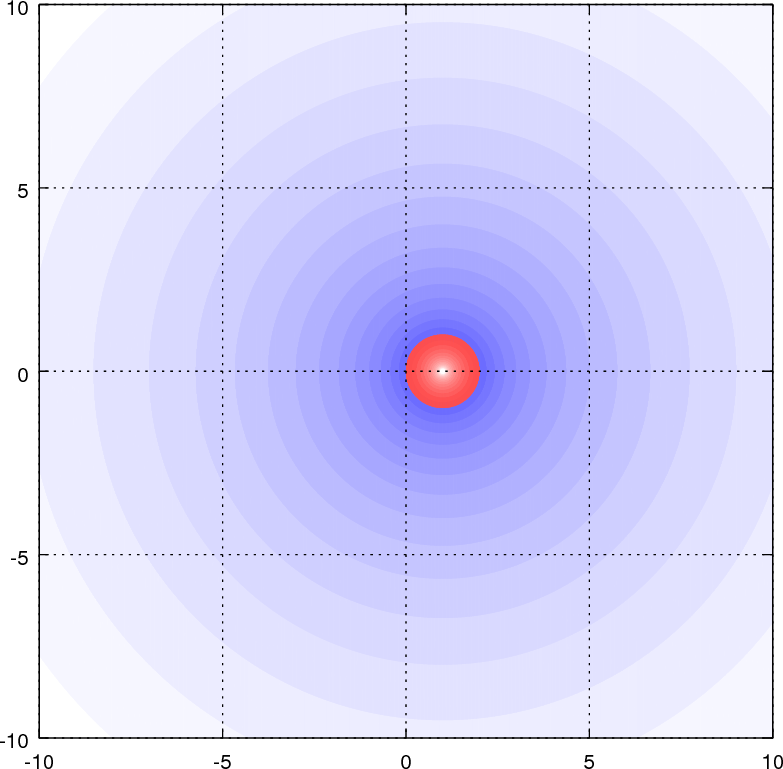
\includegraphics[width=.3\textwidth]{fig/stability-radau1}
  \hfill
  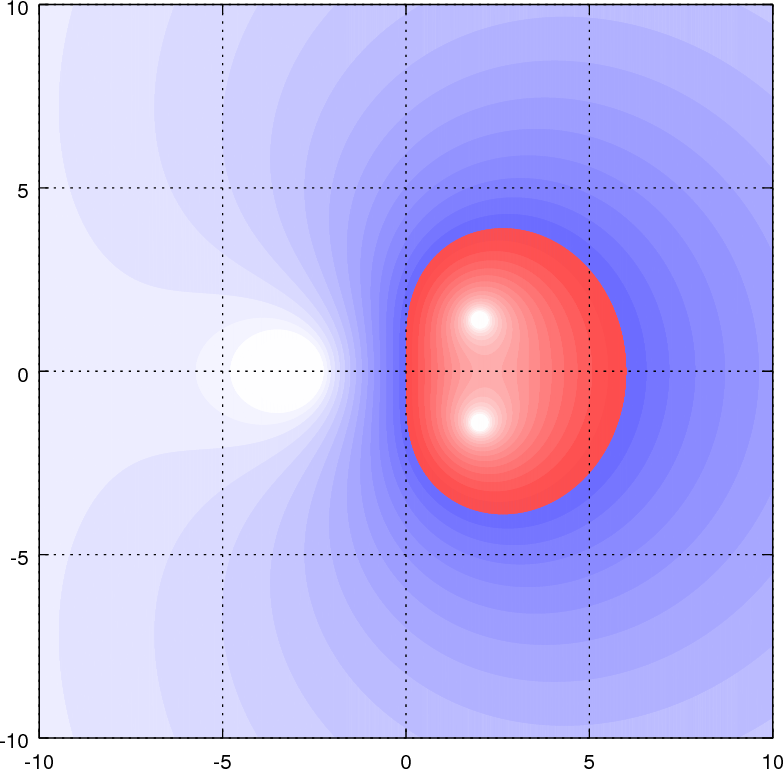
\includegraphics[width=.3\textwidth]{fig/stability-radau2}
  \hfill
  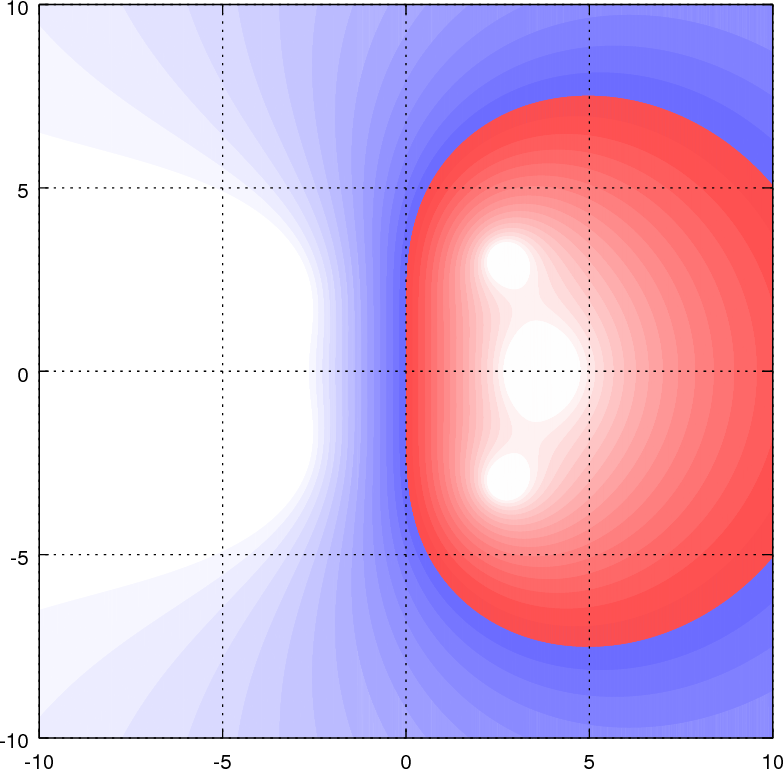
\includegraphics[width=.3\textwidth]{fig/stability-radau3}
  \caption{Stability domains of right Radau-collocation methods with
    one (implicit Euler), two, and three collocation points (left to
    right). Note the different scaling of coordinate axes in
    comparison with previous figures.}
  \label{fig:radau-collocation}
\end{figure}
%\endinput
\section{Considerations on implementation}

\begin{intro}
  Implicit Runge-Kutta methods require the solution of a nonlinear
  system of size $\rks\cdot d$, where $\rks$ is the number of stages
  and $d$ the dimension of the system of ODE. DIRK methods are simpler
  and only require the solution of a system of dimension $d$. Thus, we
  should prefer this class of methods, weren't it for
\end{intro}

\begin{Theorem}{DIRK-order-barrier}
  A B-stable DIRK method has at most order 4
\end{Theorem}

\begin{proof}
  See~\cite[Theorem 13.13]{HairerWanner10}.
\end{proof}

\begin{remark}
  In each step of an IRK, we have to solve a (non-)linear system for
  the quantities $g_i$. First, we note that in order to reduce
  round-off errors, it is advantageous to solve for $z_i = g_i-y_0$,
  since, especially for small time steps, $z_i$ is expected to be much
  smaller than $g_i$. Thus, we have to solve the system
  \begin{gather}
    \label{eq:implicit:21}
    z_i = h \sum_{j=1}^{\rks} a_{ij} f(t_0+c_jh, y_0+z_j),
    \quad
    i=1,\dots,\rks.
  \end{gather}
  Using the Runge-Kutta matrix $A$, we rewrite this as
  \begin{gather}
    \label{eq:implicit:22}
    \begin{pmatrix}
      z_1\\\vdots\\z_\rks
    \end{pmatrix}
    = A
    \begin{pmatrix}
      hf(t_0+c_1h, y_0+z_1)
      \\\vdots\\
      hf(t_0+c_\rks h, y_0+z_\rks)
    \end{pmatrix}.
  \end{gather}
  The latter can be used to avoid additional function evaluations by
  computing
  \begin{gather}
    \label{eq:implicit:23}
    y_1 = y_0 + b^TA^{-1}z, 
  \end{gather}
  which again is numerically much more stable than evaluating $f$ with
  a possibly large Lipschitz constant.
\end{remark}

%\begin{remark}
%  Each step of the Newton iteration requires the inversion of a 
%\end{remark}

%%% Local Variables: 
%%% mode: latex
%%% TeX-master: "notes"
%%% End: 
